\section{Analyse à gros grain}
\label{sec:analyse_gros_grain}

\subsection{Première experience}
L'objectif de notre première expérience est de mieux comprendre le renommage d'entités. En particulier, d'observer quand les renommages apparaissent et en quelle quantité. Nous avons donc analysé chaque périodes comme décrites plus tôt sur chaque projets de notre corpus. Nous comptons donc sur la detection automatique de renommage de Git et l'utilisons dans notre outils développé en Ruby pour obtenir notre chiffres (détails dans la section résultats). (TODO pq Ruby ?) Plus précisement nous suivons ces trois étapes entre chaque périodes:\\
\begin{enumerate}
\item On liste les fichiers existant à la fin de la période.
\item Pour chacun de ces fichiers, on extrait sa séquence de modification durant la période en activant la détection de renommage (commande \texttt{git log -M})
\item On calcule à partir des informations receuillis par exemple le pourcentage de fichiers $\%F_{R}$ qui ont étés renommés au moins une fois durant la période.
\end{enumerate}

A notre connaissance il n'existe pas d'évaluation empirique de l'algorithm utilisé par Git. Néanmoins nous procédons à une évaluation manuelle de son comportement dans la partie conclusion et nous n'avons pas noté de faux positif sur 100 renommages aléatoire récupéré par notre outil. \\

\subsubsection{Métriques et Renommage}
Un gestionnaire de versions (VCS) offre plusieurs moyens de calculer les métriques de procédés car il stocke les informations sur les entités modifiés à chaque nouvelle version, l'auteur de ces modifications, la date etc. De plus il permet la récupération du contenu de chaque entité et de l'ensemble d'un projet à une version donnée. Pour calculer ces métriques, il est donc possible d'analyser chaque entités modifiés lors d'une période puis de ne garder uniquement les entités toujours présente à la dernière version de notre période.\\
Par ailleurs, il faut noter qu'un VCS identifie une entité par son chemin + nom de fichier. On en déduit qu'un renommage du fichier ou d'un dossier, aura un impact sur le calcul des métriques. Pour expliquer cet impact, on présente un exemple d'historique d'un logiciel figure 2. Ce projet ne contient qu'une entité, Test.php, qui est renommé en Hello.php dans la dernière version. Dans cet exemple nous calculons le nombre de développeurs (NoD) entre la version 1 et 3.\\
Le NoD d'une entité de code source au cours d'une période de son histoire correspond au nombre de développeurs ayant étés identifiés comme auteurs d'une modification sur l'entité pendant la période donnée.\\

\begin{figure}[t]
	\centering
	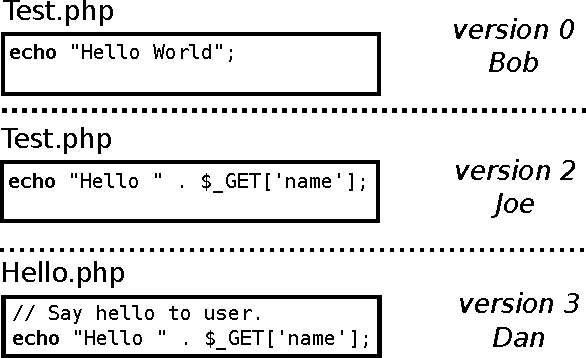
\includegraphics[width=0.8\linewidth,keepaspectratio]{data/figures/example.pdf}
	\caption{Example of a project history. The project is composed of only one file \texttt{Test.php} which is renamed to \texttt{Hello.php} in the last version.}
	\label{fig:example}
\end{figure}
Si on ne prend pas en compte le renommage, la dernière version ne contient qu'une entité. C'est donc cette entité uniquement qui sera considérée. De plus l'identité exacte de cette entité n'apparait que lors de la version 3. Le calcul des métriques est donc trivial, NoD = 1\\
Par ailleurs, si on prend en compte le fait que ce fichier a été renommé, il y a trois versions à regarder en ce qui concerne l'entité. Le premier nom du fichier était Test.php. Ce fichier à un premier autheur lors de la version 1 puis un deuxième à la version 2. Le fichier est ensuite renommé en Hello.php par un troisième autheur. Le NoD est donc de 3.

Nous avons choisi de nous concentrer sur les trois métriques de procédés identifiés plus tôt pour mesurer l'impact du renommage. En utilisant des scripts Ruby pour mesurer les métriques sur nos projets, voici plus précisement comment nous avons procédés:

Nous récupérons d'abord la dernière version du projet pour obtenir les entités existante à la fin de la période considéréé. On note $A$ cet ensemble d'entités. Deuxièmement, toujours grace aux commandes git, nous récupérons toute les modifications effectués durant la période. On note $C$ l'ensemble des modifications dans l'ordre chronologique. Troisièmement nous parcourons cet ensemble de modification en commencant par la plus ancienne ($c_0 \in C$) jusqu'à la plus récente  ($c_n \in C$) dans le but de calculer les métriques de procédés pour chaque entités. On note $\mu_{a}^{M}$ la valeur de la métrique $M$ pour l'entité $a$. Ensuite nous calculons les métriques comme suivant (on note $c_i$ la modification courante lors du parcours): 

\begin{description}
	\item[NoD] (nombre de développeurs) Pour chaque entité $a$ pointé par $c_i$ qui appartient aussi à $A$ ($a \in A$), on ajoute à $\mu_{a}^{NoD}$ le nombre d'autheurs qui ont effectués les modifications $c_i$ et qui ont modifiés $a$ pour la première fois dans la période.
	\item[NoC] (nombre de modifications) Pour chaque entité $a$ pointé par $c_i$ qui appartient aussi à $A$ ($a \in A$), on ajoute $1$ à $\mu_{a}^{C}$ tels que $c_i$ indique qu'une nouvelle modification a été effectuée.
	\item[CC] (Code Churn) Pour chaque entité $a$ pointé par $c_i$ qui appartient aussi à $A$ ($a \in A$), on vérifie d'abord que la modification n'est pas une creation d'entité. Si c'est le cas celà veut dire que l'entité a été crée durant la période, donc on initialise son $\mu_{a}^{CC}$ à son nombre de lignes. Ensuite au prochain $c_j$ qui cible $a$ dans la période avec ($i < j$), on compare les deux versions et on ajoute à $\mu_{a}^{CC}$ le nombre de lignes ajoutés ou suprimés.
\end{description}


\subsection{deuxième expérience}

Le but de la deuxième expérience est de voir si le renommage peut biaiser significativement les valeurs des métriques de procédés décrites ci dessus. Pour ca, nous effectuons une analyse dans le pire des cas. On sélectionne la période de nos projets qui a la plus grande valeurs de fichiers renommés en excluant la période initiale qui n'est généralement pas observé dans les études. Nous calculons ensuite les trois métriques avec et sans le renommage de fichiers pris en compte, puis nous calculons la correlation de coéficient de Spearman entre les métriques avec et sans la detection de renommage. Un gros coéficient, proche de $1$, indiquera que les métriques avec et sans détection de renommage sont très similaires alors qu'un coéficient plus petit, 0.5 et moins, indiquera que les métriques avec et sans détection de renommage sont très différentes.\\
